\documentclass[a4paper,14pt]{extreport} % формат документа

\usepackage{amsmath}
\usepackage{cmap} % поиск в ПДФ
\usepackage[T2A]{fontenc} % кодировка
\usepackage[utf8]{inputenc} % кодировка исходного текста
\usepackage[english,russian]{babel} % локализация и переносы
\usepackage[left = 2cm, right = 1cm, top = 2cm, bottom = 2 cm]{geometry} % поля
\usepackage{listings}
\usepackage{graphicx} % для вставки рисунков
\usepackage{amsmath}
\usepackage{float}
\usepackage{multirow}
\graphicspath{{img/}}
\DeclareGraphicsExtensions{.pdf,.png,.jpg}
\newcommand{\anonsection}[1]{\section*{#1}\addcontentsline{toc}{section}{#1}}

\lstset{ %
	language=Lisp,                % Язык программирования 
	numbers=left,                   % С какой стороны нумеровать          
	frame=single,                    % Добавить рамку
}

\begin{document}
\begin{titlepage}

    \begin{table}[H]
        \centering
        \footnotesize
        \begin{tabular}{cc}
            \multirow{8}{*}{
\includegraphics[scale=0.35]{bmstu.jpg}}
            & \\
            & \\
            & \textbf{Министерство науки и высшего образования Российской Федерации} \\
            & \textbf{Федеральное государственное бюджетное образовательное учреждение} \\
            & \textbf{высшего образования} \\
            & \textbf{<<Московский государственный технический} \\
            & \textbf{университет имени Н.Э. Баумана>>} \\
            & \textbf{(МГТУ им. Н.Э. Баумана)} \\
        \end{tabular}
    \end{table}

    \vspace{-2.5cm}

    \begin{flushleft}
        \rule[-1cm]{\textwidth}{3pt}
        \rule{\textwidth}{1pt}
    \end{flushleft}

    \begin{flushleft}
        \small
        ФАКУЛЬТЕТ
        \underline{<<Информатика и системы управления>>\ \ \ \ \ \ \ 
        \ \ \ \ \ \ \ \ \ \ \ \ \ \ \ \ \ \ \ \ \ \ \ \ \ \ \ \ \ \ \ 
    \ \ \ \ \ \ \ \ \ \ \ \ \ \ \ } \\
        КАФЕДРА
        \underline{<<Программное обеспечение ЭВМ и
        информационные технологии>>
        \ \ \ \ \ \ \ \ \ \ \ \ \ \ \ \ \ \ \ \ }
    \end{flushleft}

    \vspace{2cm}

    \begin{center}
        \textbf{Лабораторная работа № 4} \\
        \vspace{0.5cm}
    \end{center}

    \vspace{4cm}

    \begin{flushleft}
        \begin{tabular}{ll}
            \textbf{Дисциплина} & Экономика программной инженерии.  \\
            \textbf{Тема} & Актуализация параметров проекта. \\
            & Ввод фактических данных для \\
            & задач и просмотр отклонений от контрольного плана \\
            \\
            \textbf{Студент} & Сиденко А.Г. \\
            \textbf{Группа} & ИУ7-83Б \\
            \textbf{Оценка (баллы)} & \\
            \textbf{Преподаватель} & Барышникова М.Ю., Силантьева А.В.   \\
        \end{tabular}
    \end{flushleft}

    \vspace{4cm}

   \begin{center}
        Москва, 2021 г.
    \end{center}

\end{titlepage}

\begin{enumerate}

\item \textbf{Основное задание}

Содержание проекта: Команда разработчиков из 16 человек занимается созданием карты города на основе собственного модуля отображения. Проект должен быть завершен в течение 6 месяцев. Бюджет проекта: 50 000 рублей.

\item \textbf{Задайте дату отчета (9 апреля).}

\begin{figure}[H]
  \centering
  \caption{Дата отчета. }
  
\includegraphics[scale=1]{1}
\end{figure}

\item \textbf{Внесите фактические данные для отдельных задач проекта (по заданию преподавателя).}

Отметить как выполненные все работы, которые должны были завершиться на эту дату, кроме:
6 -- на неделю позже закончилась

13 -- 260 человекочасов

15 -- началась на неделю позже

9 -- выполнена на 50\%

С 1 апреля аренда сервера на 5 \% больше

3д аниматор на 10 дней уехал на повышение квалификации с 15 марта, после увеличение зп на 10\%, но далее задействован в проекте на 80\%

Программист 1 уволился с 1 апреля

И с 1 апреля начальники потребовали на 20 рублей бумаги, чтобы печатать на совещания.

\newpage

Повышаем аренду сервера:

\begin{figure}[H]
  \centering
  \caption{Аренда сервера. }
  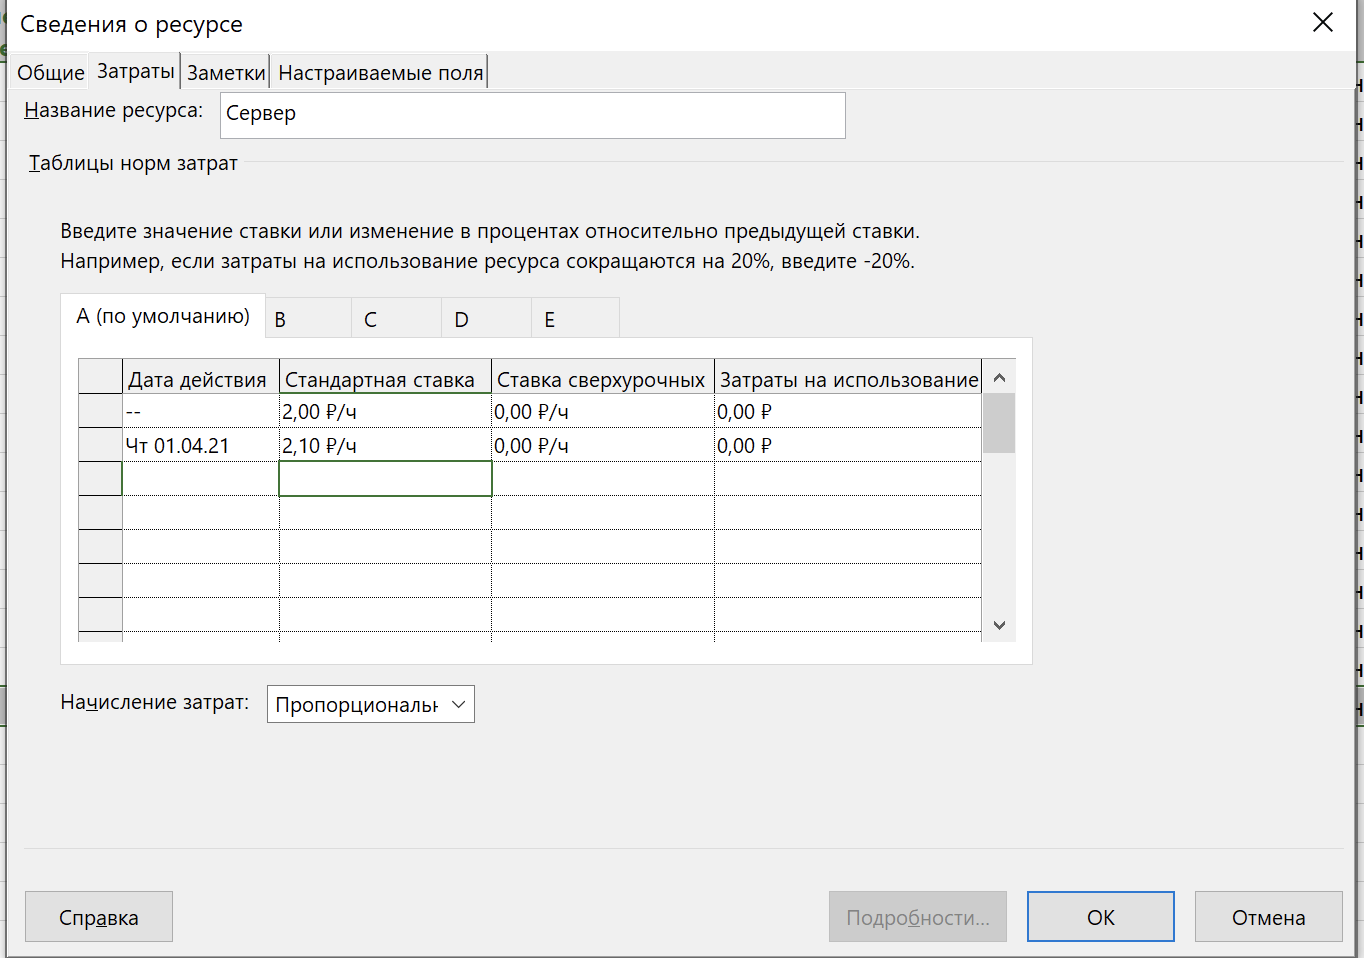
\includegraphics[scale=0.7]{2}
\end{figure}

Далее отправляем аниматора на повышение квалификации и после увеличиваем его заработную плату.

\begin{figure}[H]
  \centering
  \caption{Повышение квалификации. }
  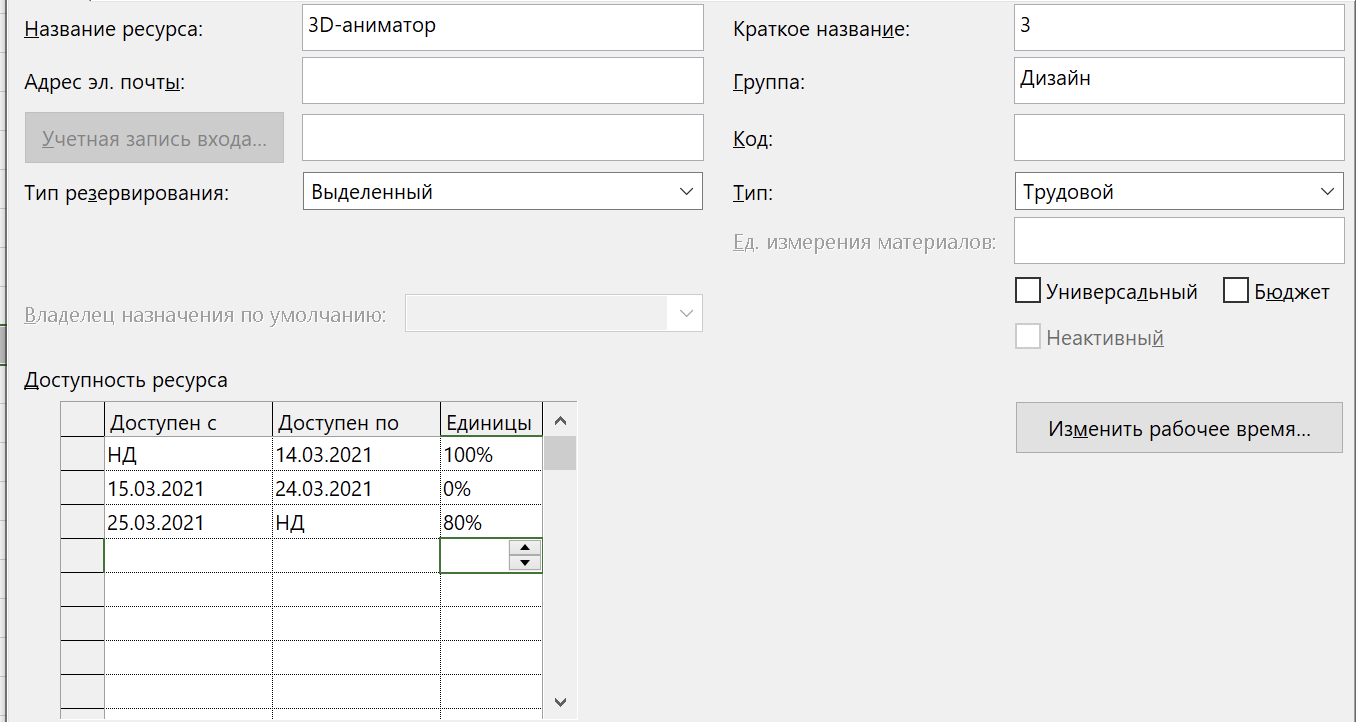
\includegraphics[scale=0.7]{3}
\end{figure}

\begin{figure}[H]
  \centering
  \caption{Повышение зп. }
  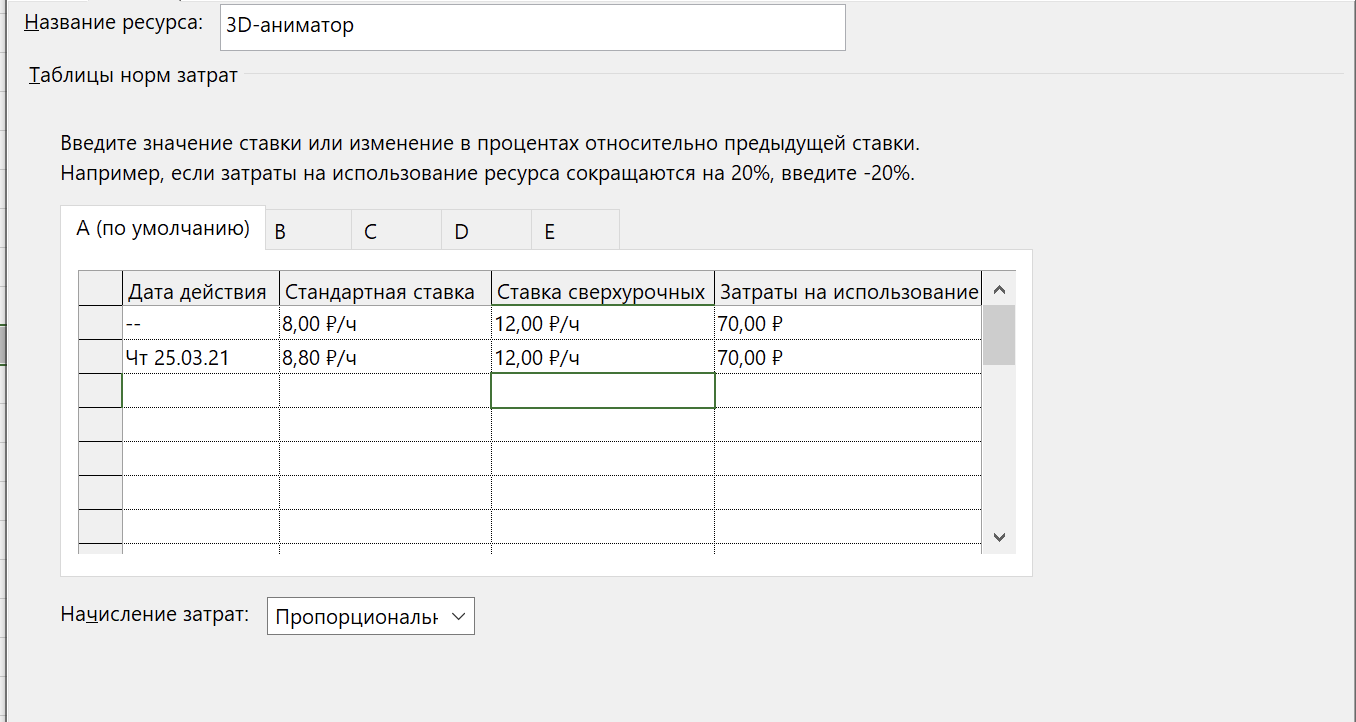
\includegraphics[scale=0.7]{6}
\end{figure}

У нас возникла перегрузка.

\begin{figure}[H]
  \centering
  \caption{Перегрузка. }
  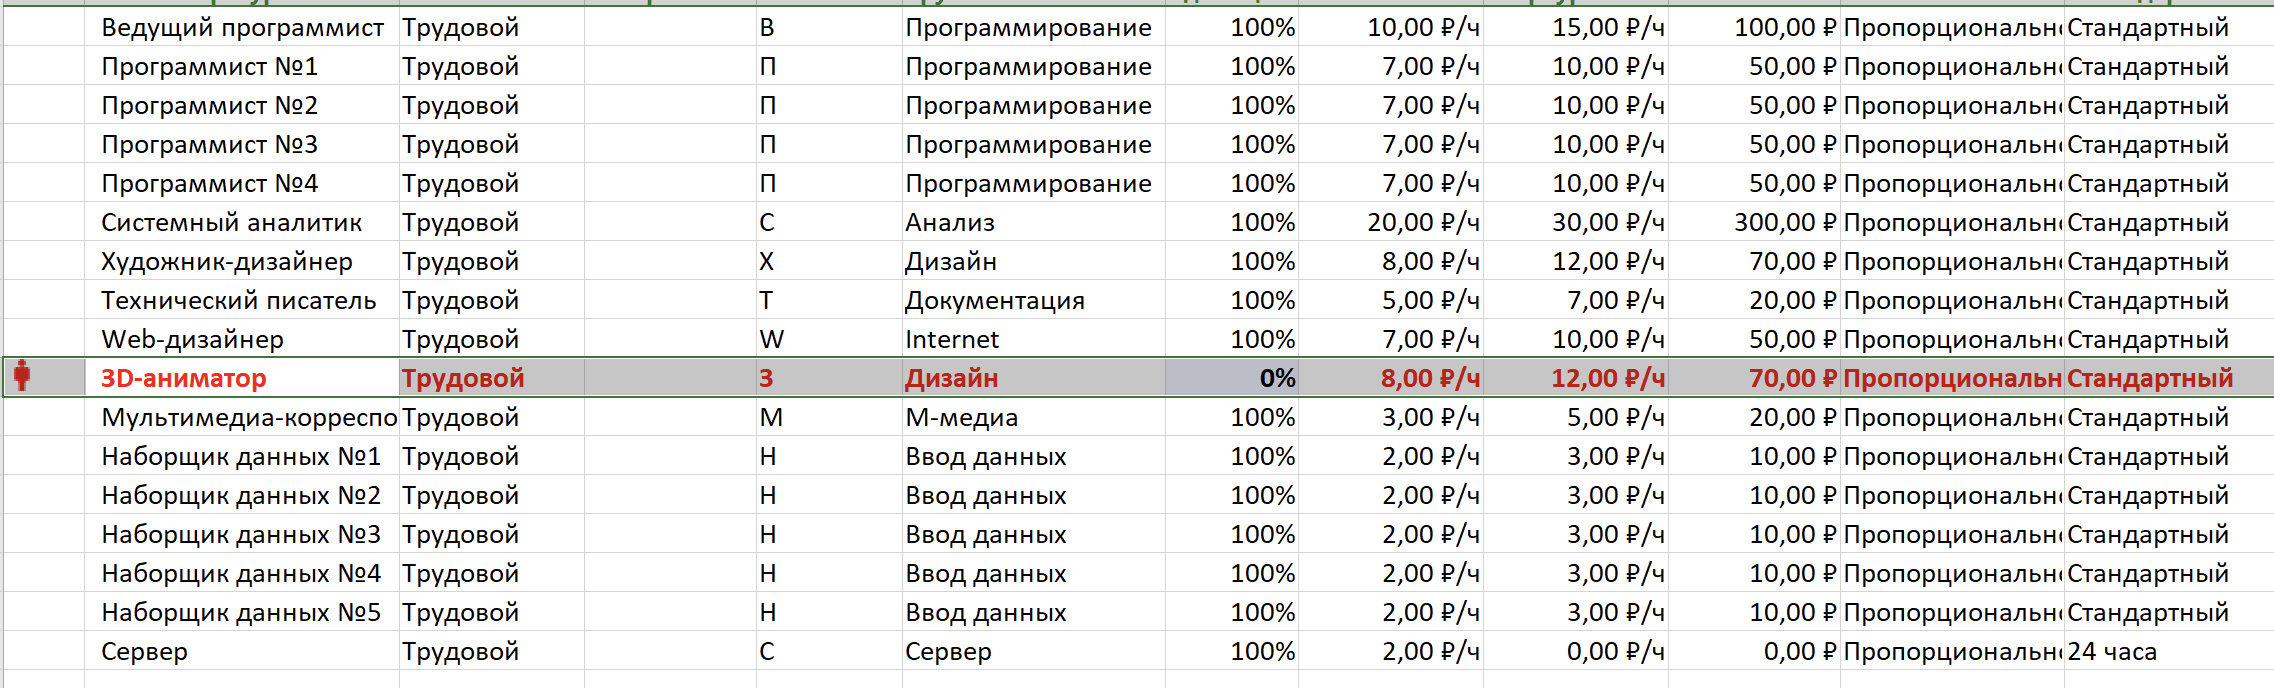
\includegraphics[scale=0.5]{4}
\end{figure}

Освобождаем его от совещаний на данный период.

\begin{figure}[H]
  \centering
  \caption{Совещания. }
  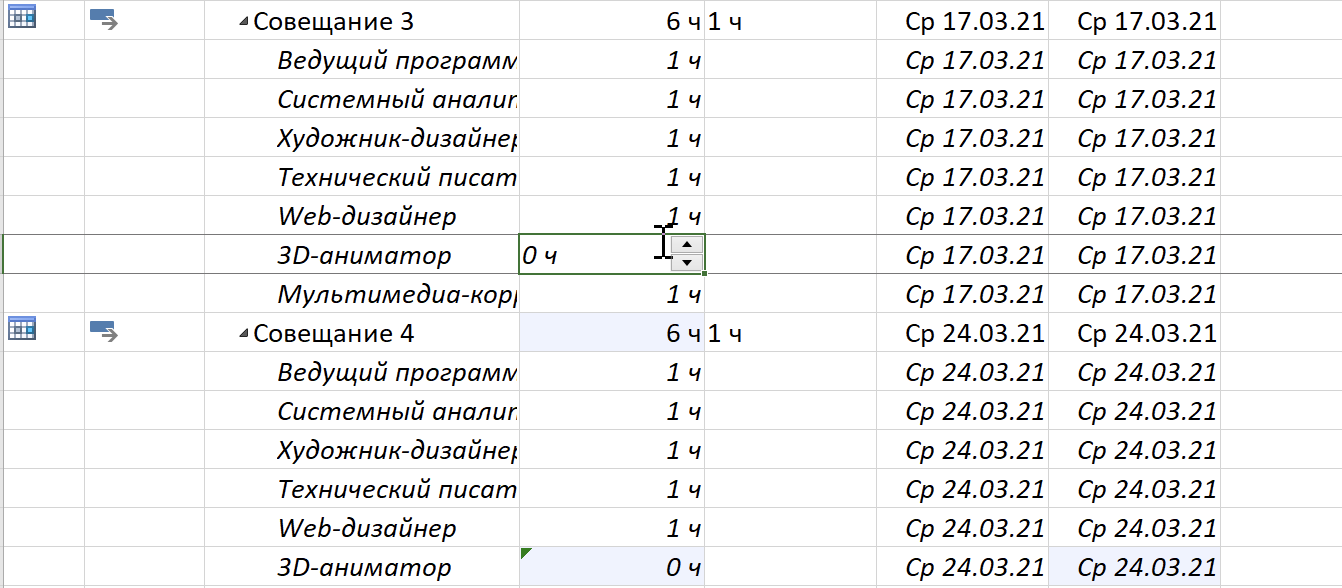
\includegraphics[scale=0.7]{5}
\end{figure}

Срок задач сдвинулся автоматически.

\begin{figure}[H]
  \centering
  \caption{Срок задач. }
  
\includegraphics[scale=0.5]{8}
\end{figure}

Программист 1 уволился с 1 апреля.

\begin{figure}[H]
  \centering
  \caption{Уволился программист. }
  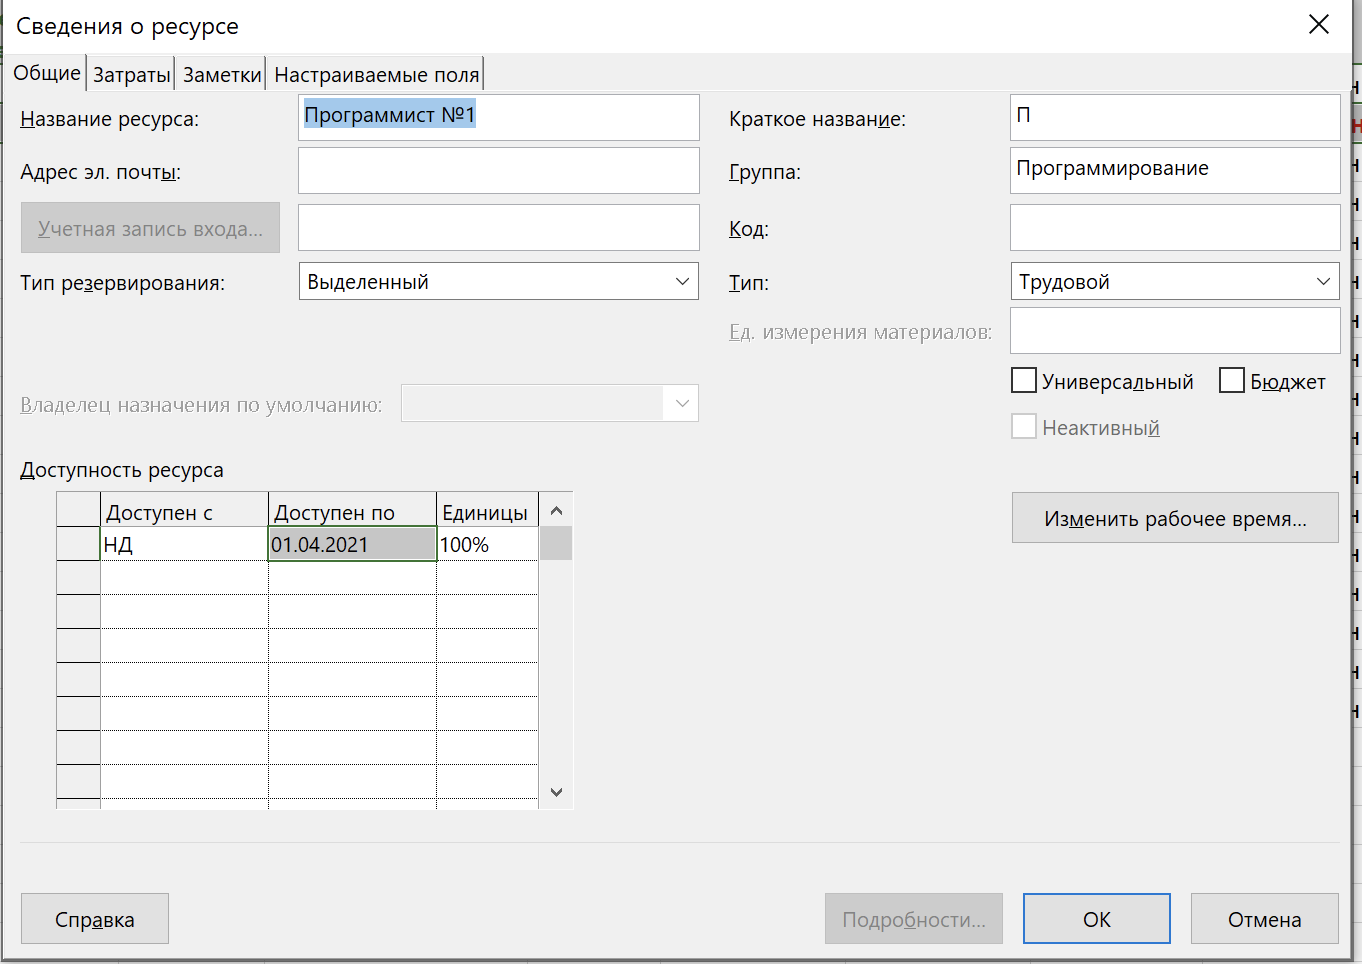
\includegraphics[scale=0.5]{7}
\end{figure}

Решаем возникшие перегрузки, ручным перераспределением ресурсов на других программистов, также увеличивается длительность выполнения задач.

\begin{figure}[H]
  \centering
  \caption{Перегрузка программиста 1. }
  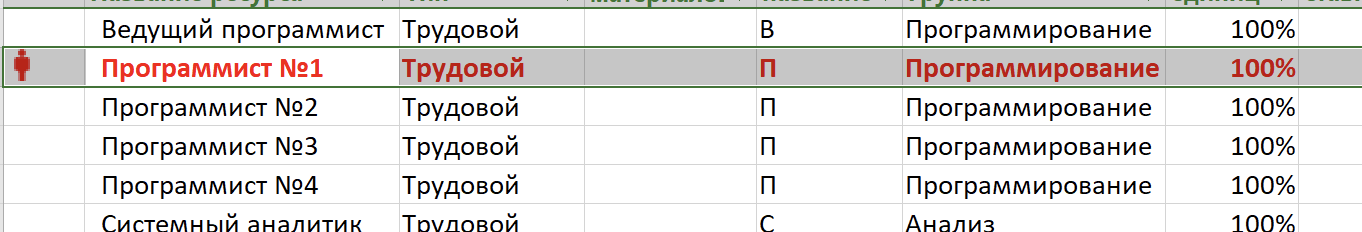
\includegraphics[scale=0.5]{10}
\end{figure}

\begin{figure}[H]
  \centering
  \caption{Перегрузка ресурсов. }
  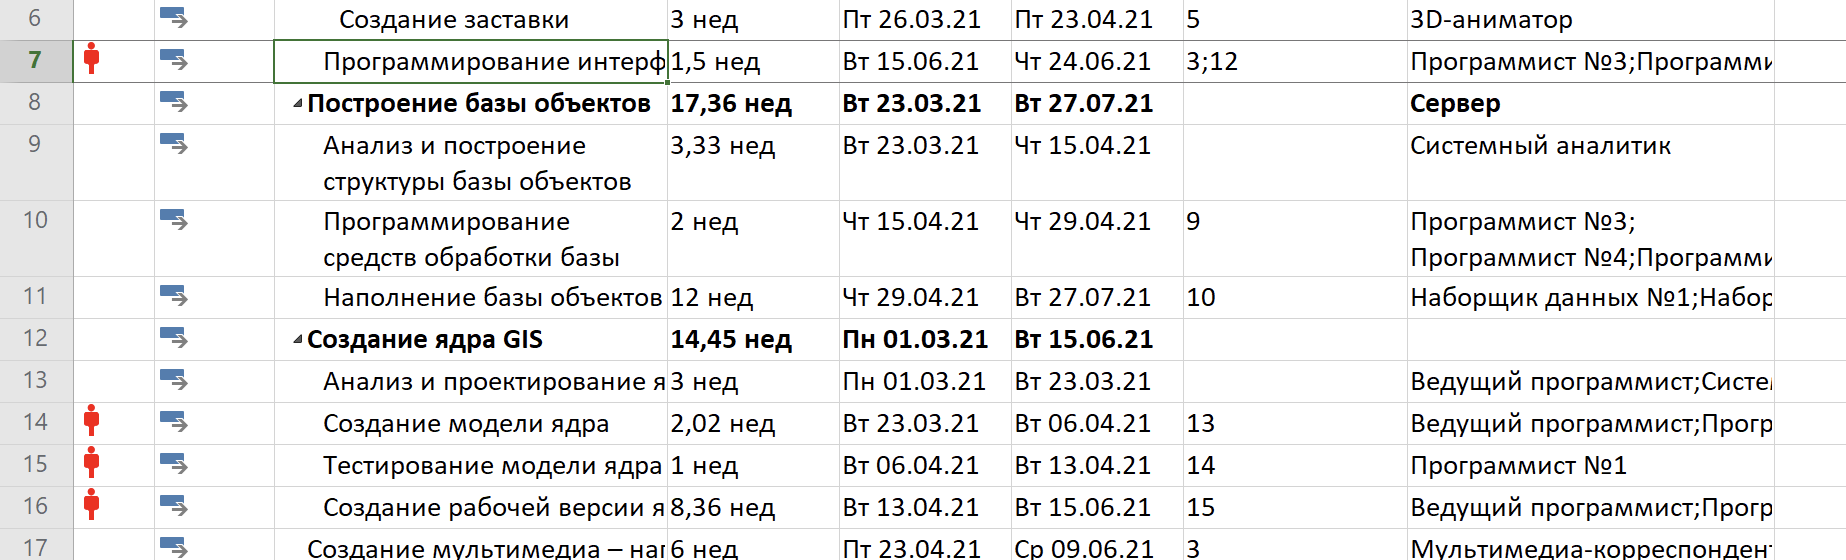
\includegraphics[scale=0.5]{9}
\end{figure}

Добавляем ресурс -- бумагу на совещания.

\begin{figure}[H]
  \centering
  \caption{Бумага. }
  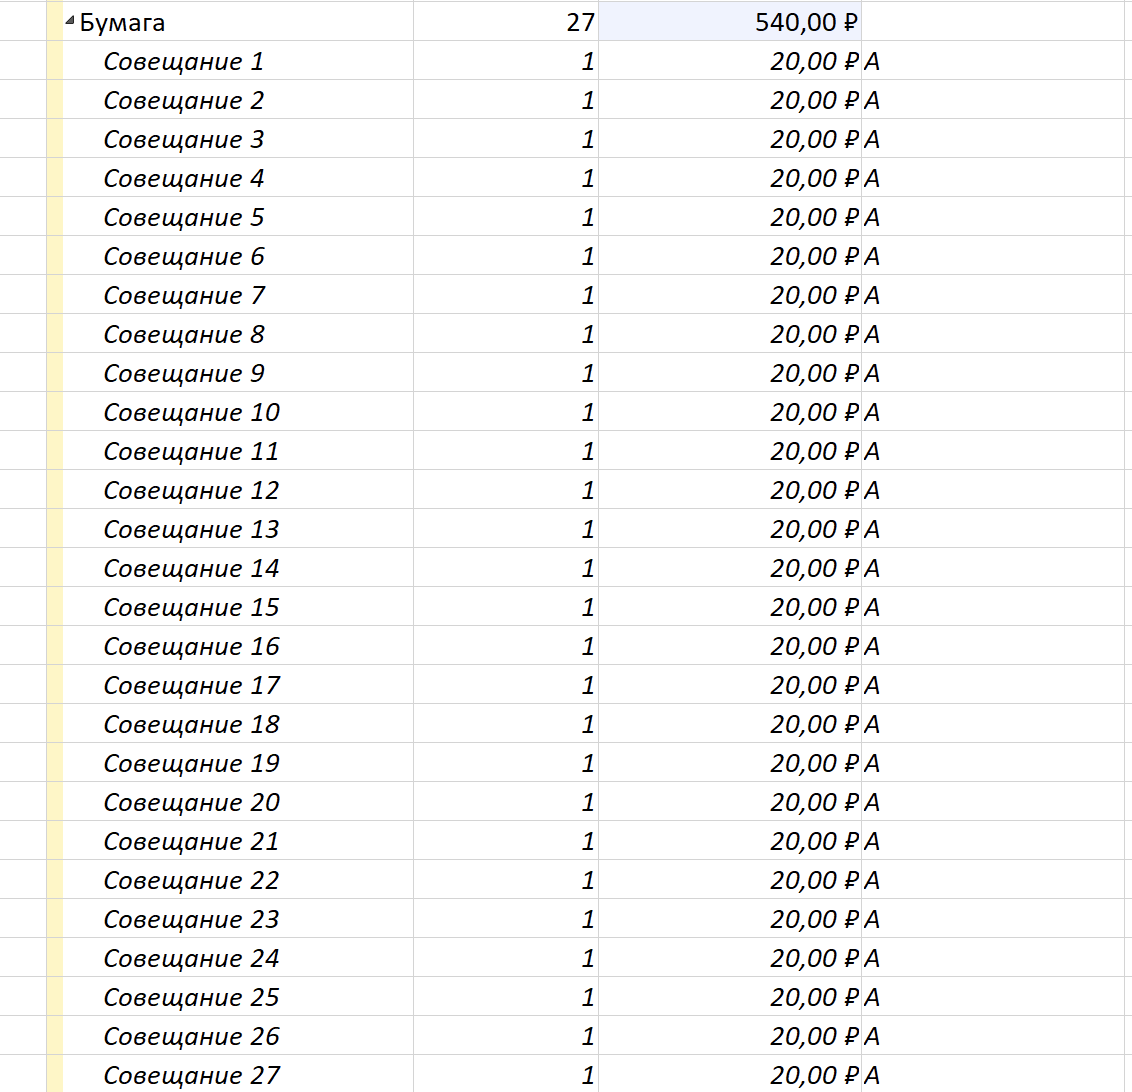
\includegraphics[scale=0.5]{11}
\end{figure}

Отмечаем как выполненные все работы, 6 -- срок окончания на неделю позже, 15 -- начало на неделю позже, 13 -- устанавливаем 260 человекочасов.

\begin{figure}[H]
  \centering
  \caption{Сдвигаем начало. }
  
\includegraphics[scale=0.7]{12}
\end{figure}

\begin{figure}[H]
  \centering
  \caption{Устанавливаем трудозатраты. }
  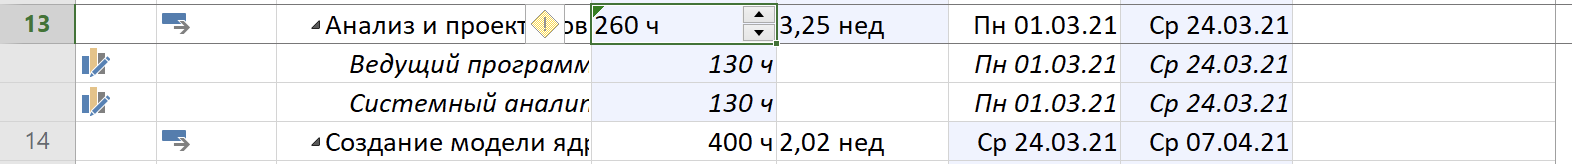
\includegraphics[scale=0.5]{13}
\end{figure}

После этого получаем.

\begin{figure}[H]
  \centering
  \caption{Итог после выполнения всех заданий. }
  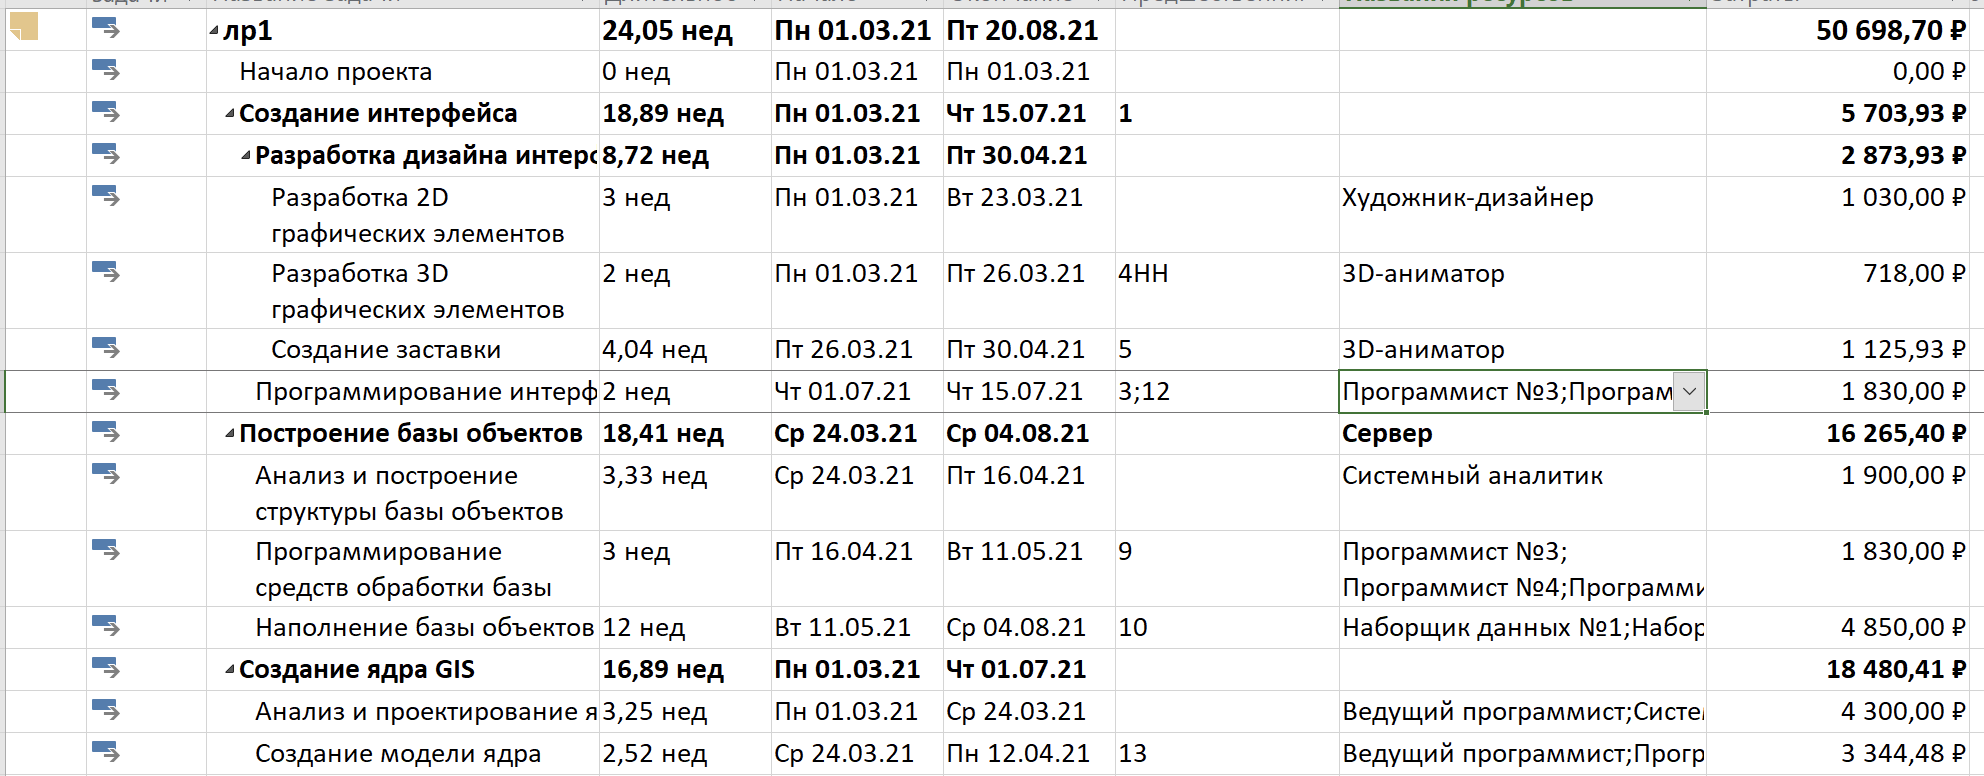
\includegraphics[scale=0.5]{14}
\end{figure}

Срок окончания сдвигается с 27 июля до 20 августа. Затраты с 48781,79 рублей до 50698,7.

Если срок окончания еще укладывается во временные рамки, то затраты совсем нет. Попробуем исправить.

Выведем отклонение по срокам.

\begin{figure}[H]
  \centering
  \caption{Отлонение по срокам. }
  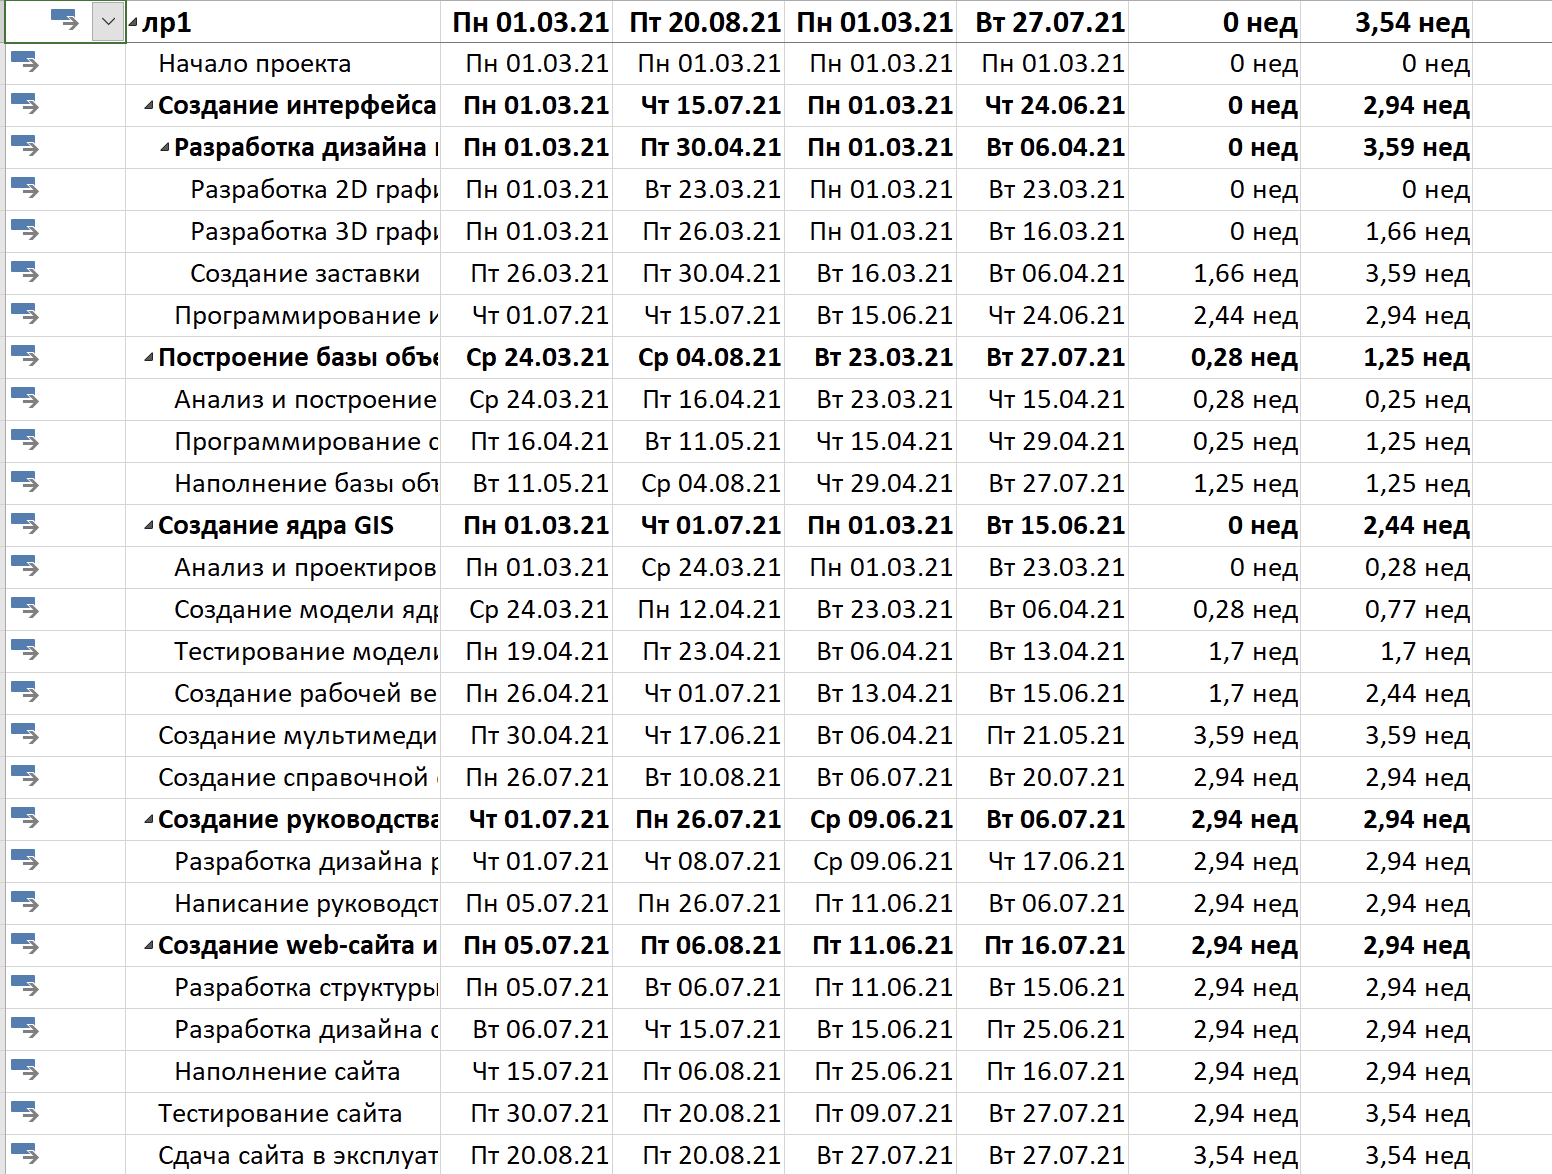
\includegraphics[scale=0.5]{15}
\end{figure}

Выведем на экран линию прогресса.

\begin{figure}[H]
  \centering
  \caption{Линия хода выполнения. }
  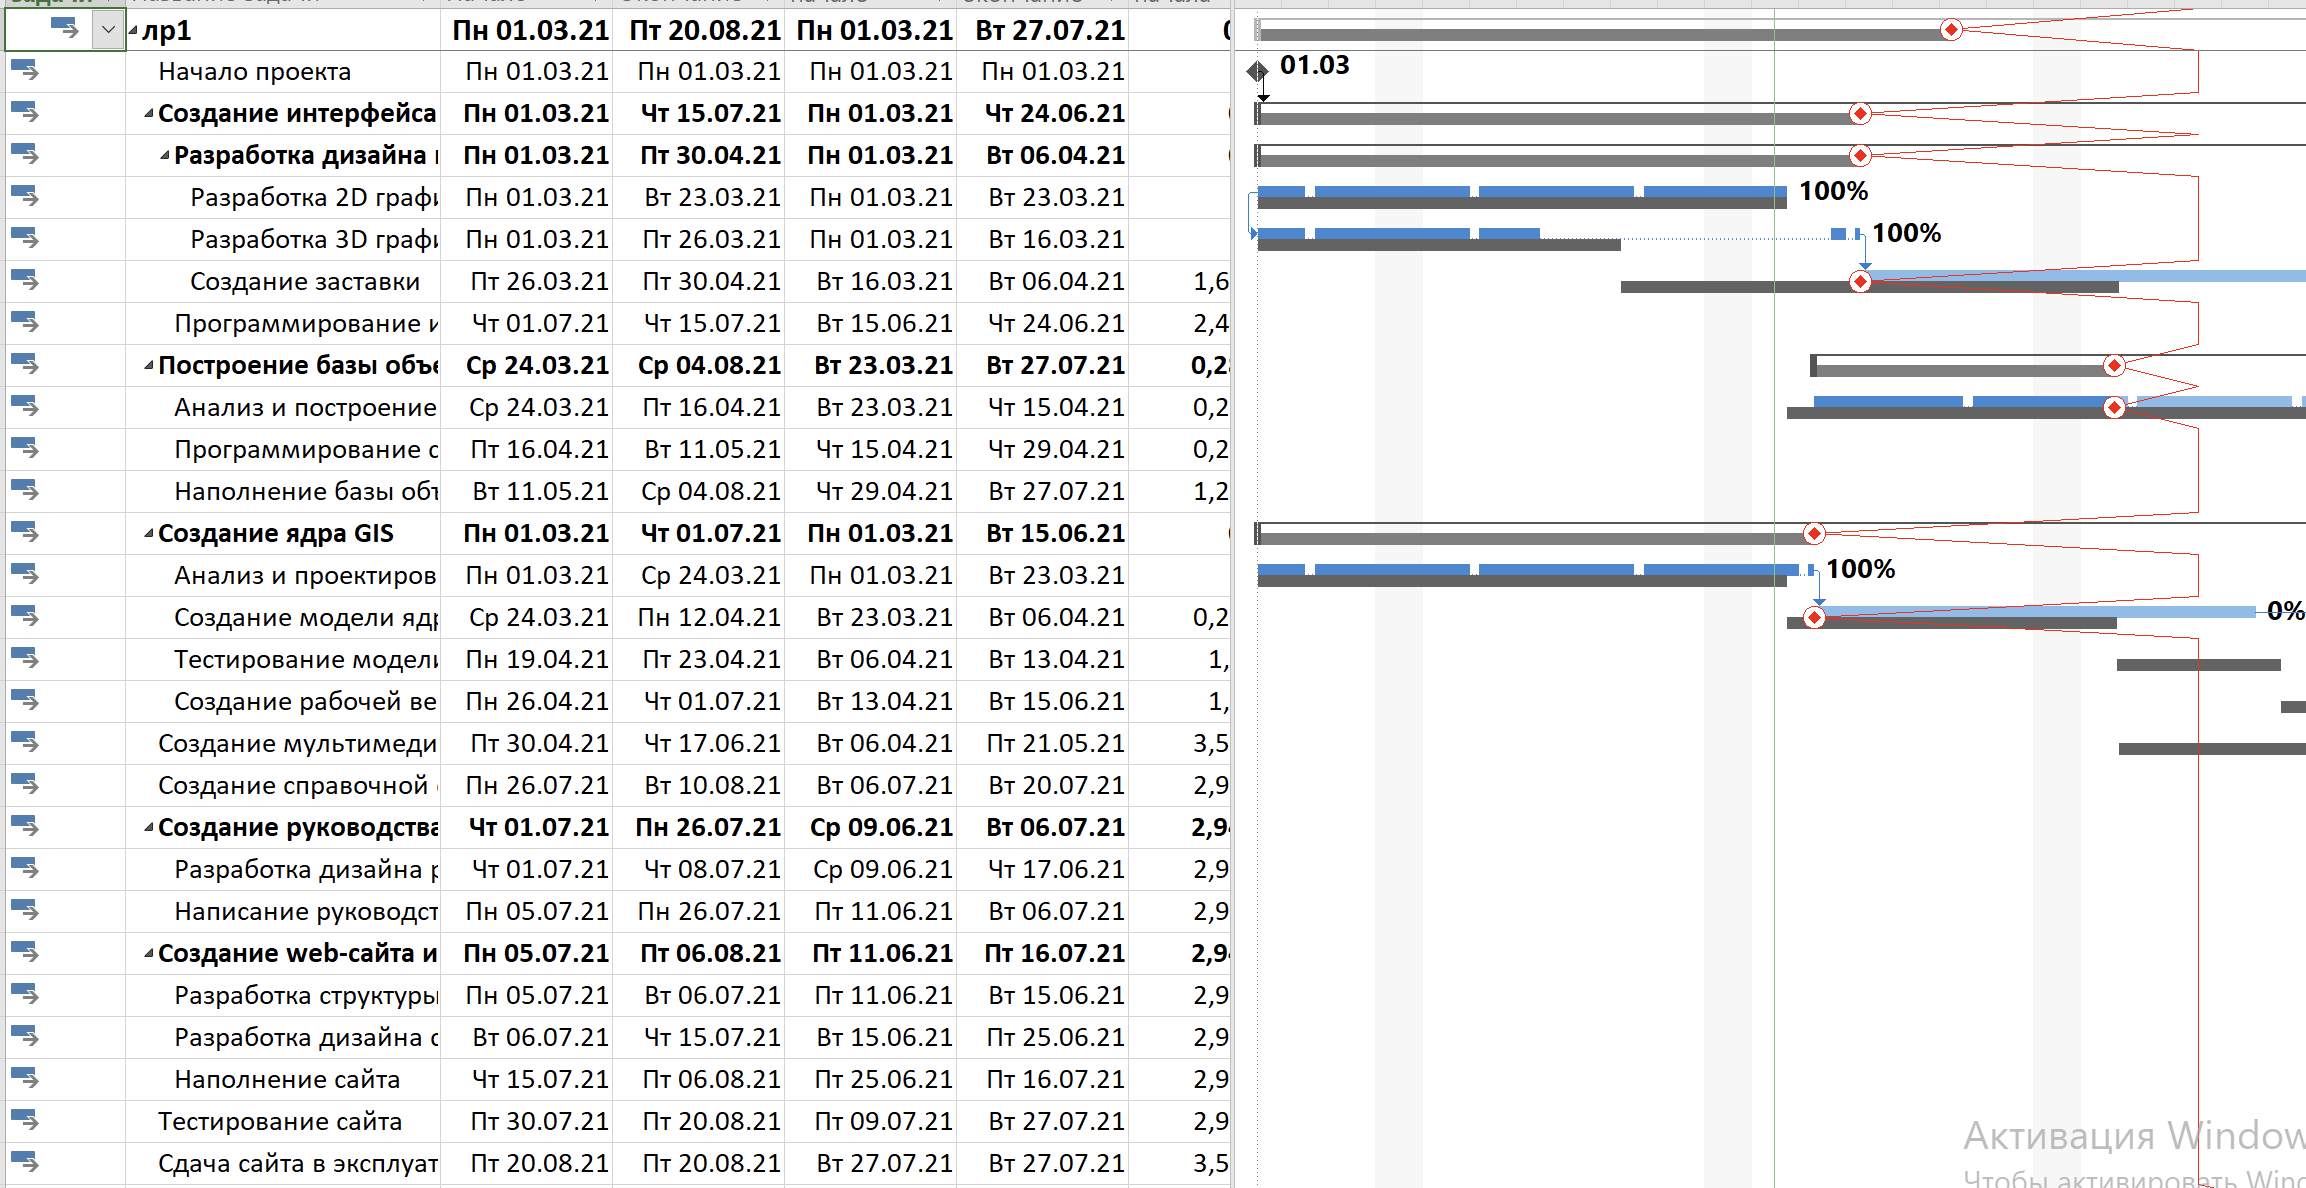
\includegraphics[scale=0.4]{17}
\end{figure}

Как видно все задачи опаздывают, имеет V-образный изгиб влево.

Как видим самое большое отклонение из-за повышения квалификации аниматора и увольнения программиста. Давайте наймем стажера в проект, до повышения его аниматор обучит. И дополнительного программиста с 1 апреля.

\begin{figure}[H]
  \centering
  \caption{Новые ресурсы. }
  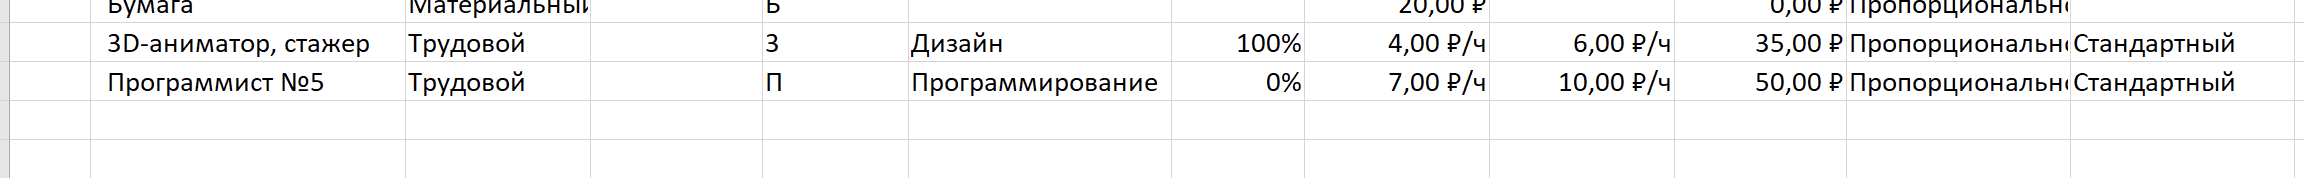
\includegraphics[scale=0.5]{16}
\end{figure}

Итого получаем.

\begin{figure}[H]
  \centering
  \caption{Итог. }
  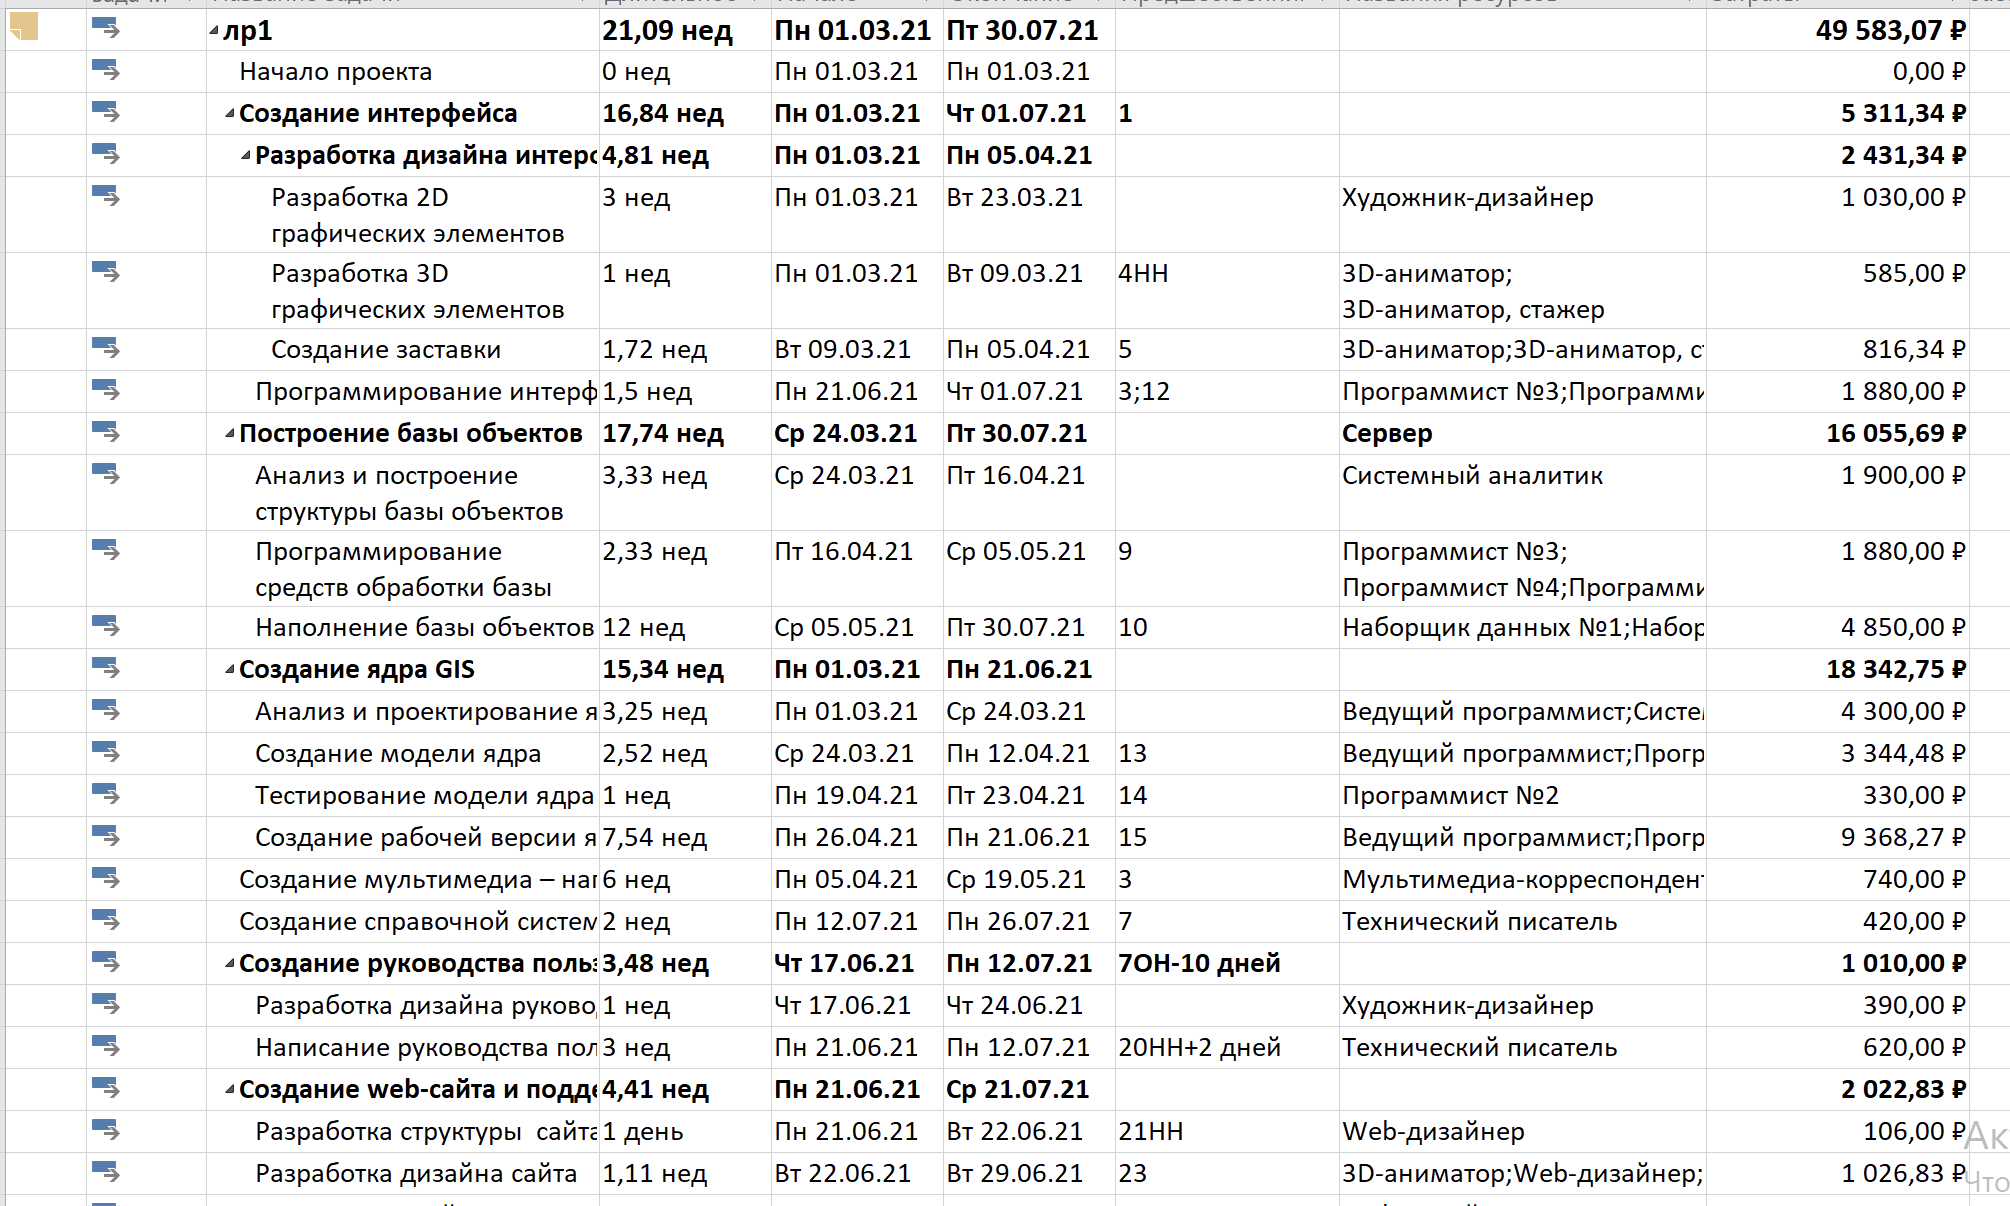
\includegraphics[scale=0.5]{18}
\end{figure}

Выведем на экран линию прогресса.

\begin{figure}[H]
  \centering
  \caption{Линия хода выполнения. }
  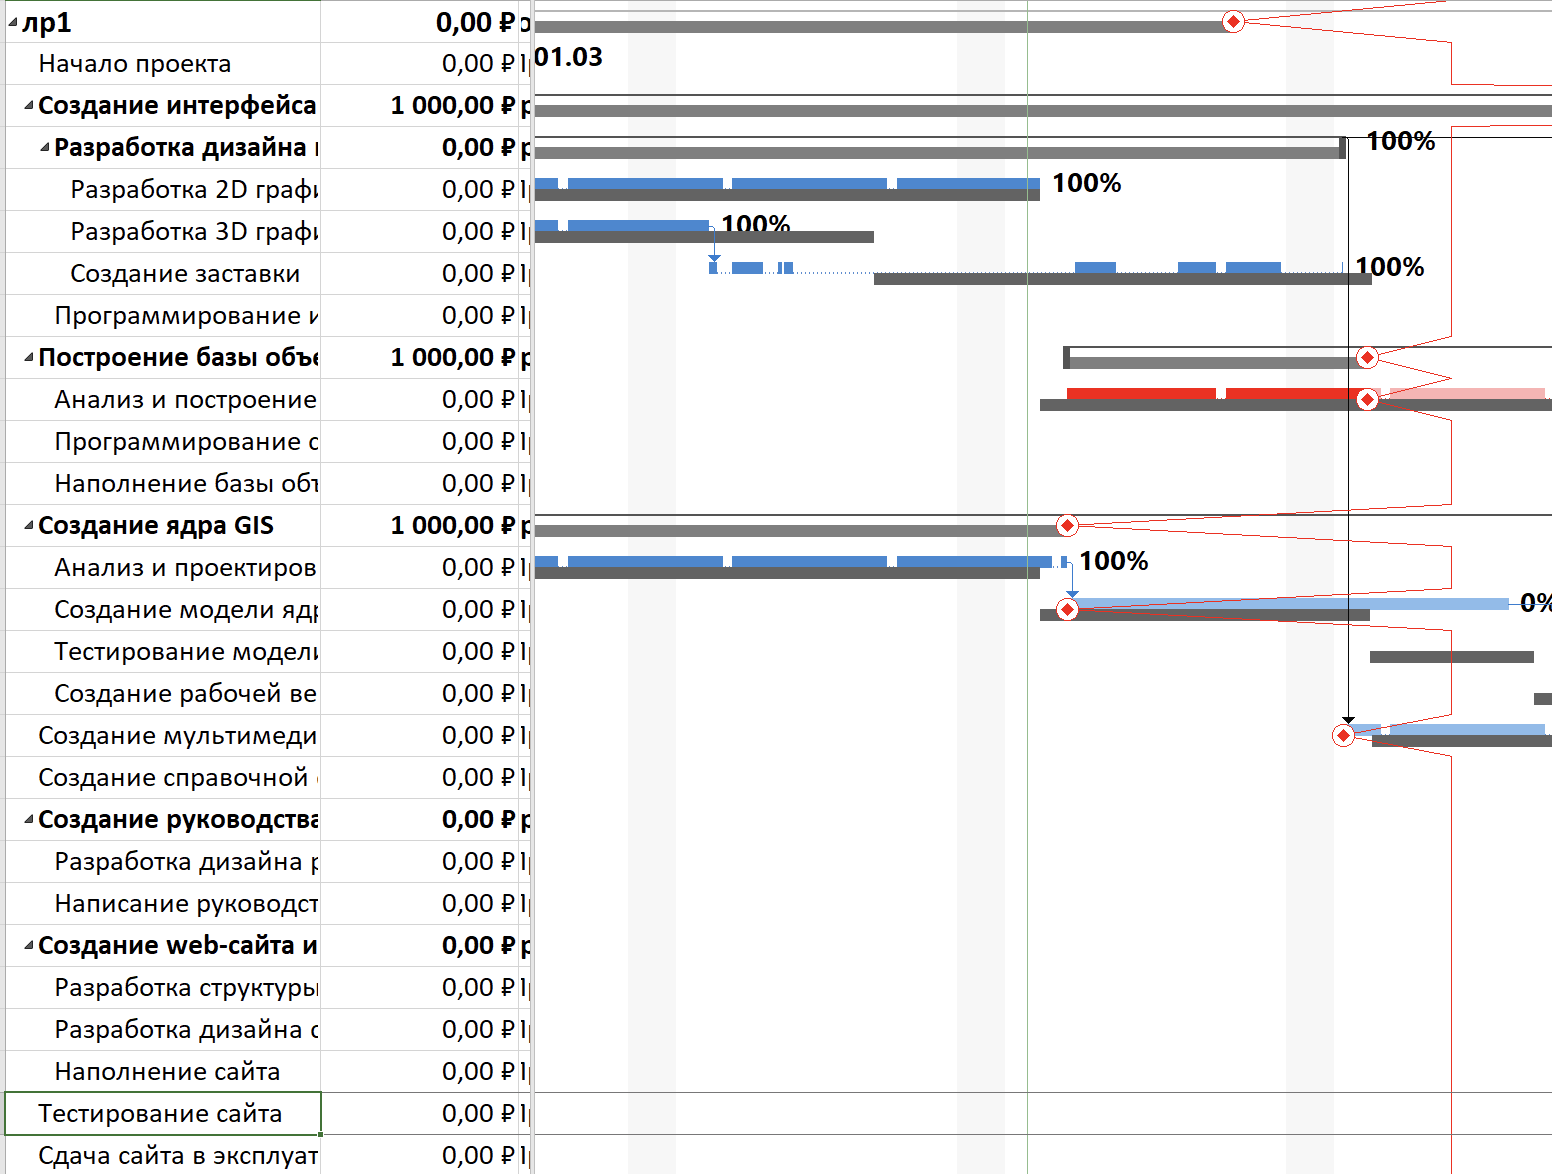
\includegraphics[scale=0.5]{19}
\end{figure}

Как видим сдвиг по строкам на 1 день вышел, а по затратам на 800 рублей.

Если посмотреть на отклонение по затратам.

\begin{figure}[H]
  \centering
  \caption{Отклонение по затратам. }
  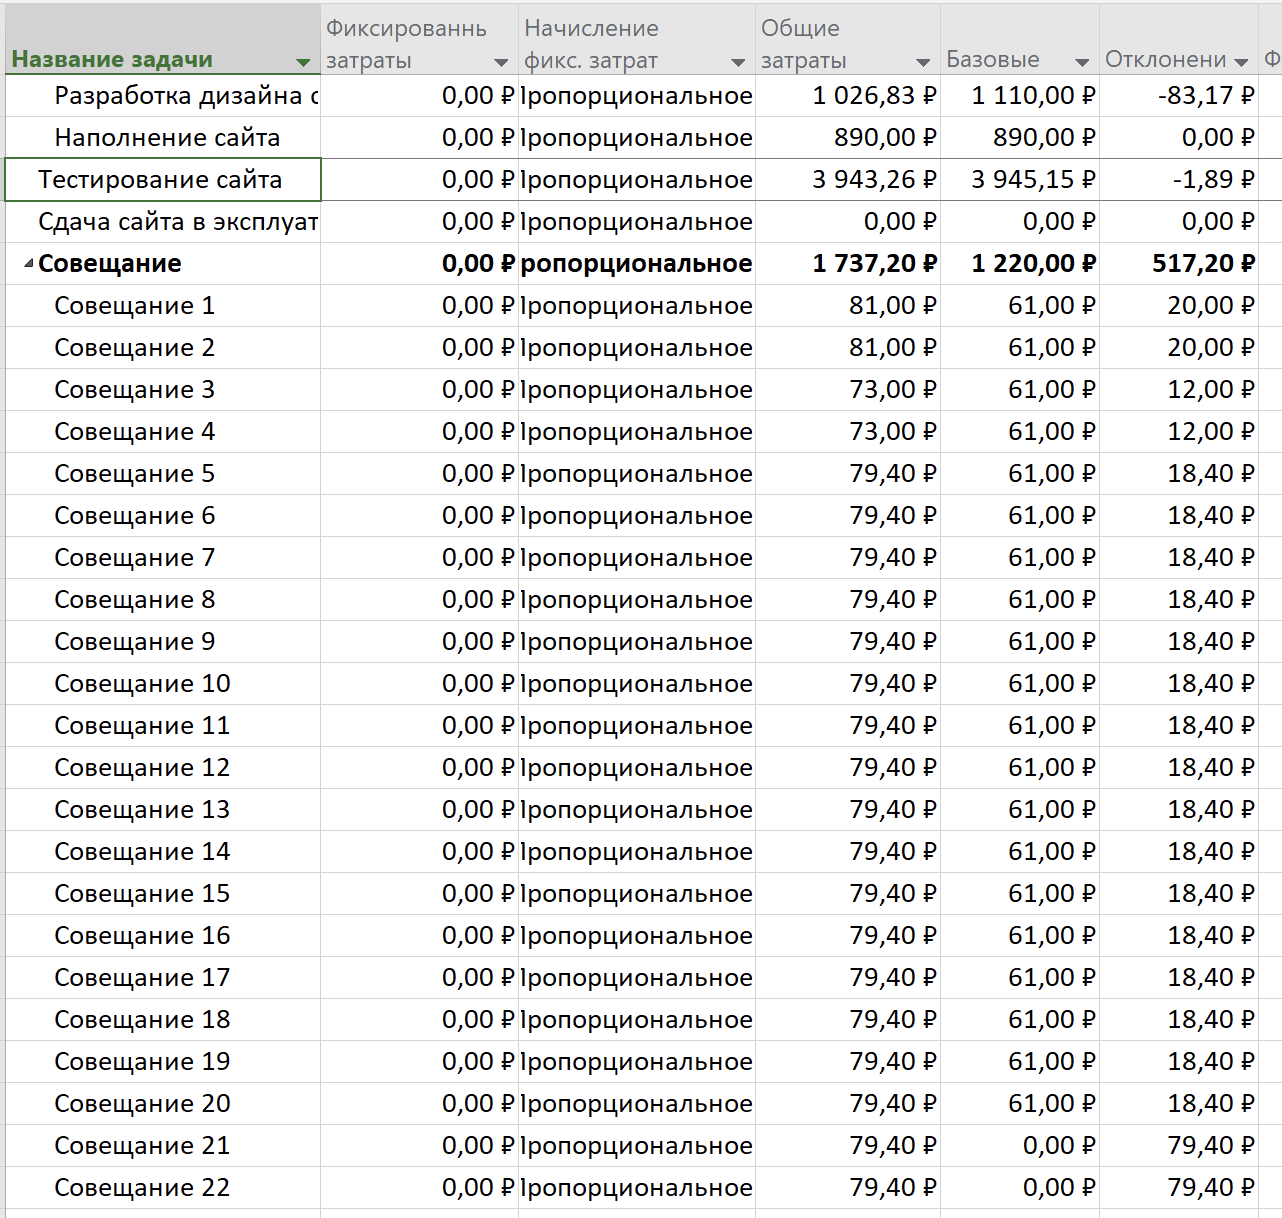
\includegraphics[scale=0.5]{20}
\end{figure}

Самые большие затраты на совещания, это на бумагу. Возможно стоит потратиться и купить новый проетор, который пригодится не только в этом, но и будущих проектах.


\end{enumerate}

\end{document}